\documentclass[a4,11pt]{article}

\usepackage[utf8]{inputenc}
\usepackage{color}
\usepackage{listings}
\lstset{xleftmargin=3em}
\lstset{
  mathescape=true,
  language=[Objective]{Caml},
  basicstyle=\ttfamily,
  extendedchars=true,
  showstringspaces=false,
  aboveskip=\smallskipamount,
  % belowskip=\smallskipamount,
  columns=fullflexible,
  moredelim=**[is][\color{blue}]{/*}{*/},
  moredelim=**[is][\color{green!60!black}]{/!}{!/},
  moredelim=**[is][\bfseries]{/(}{)/},
  moredelim=[is][\color{red}]{/[}{]/},
  breaklines=true
}
\usepackage[dvipsnames]{xcolor}
\usepackage{graphicx}
\graphicspath{ {./images/} }


\newcommand{\hb}{\texttt{\color{blue}hb}}
\newcommand{\eco}{\texttt{\color{red}eco}}
\newcommand{\rmw}{\texttt{\color{Brown}rmw}}
\newcommand{\rb}{\texttt{\color{red}rb}}
\newcommand{\mo}{\texttt{\color{Dandelion}mo}}
\newcommand{\psc}{\texttt{\color{Maroon}psc}}
\newcommand{\po}{\texttt{\color{Periwinkle}po}}
\newcommand{\rf}{\texttt{\color{Green}rf}}

\title{Research internship report}

\author{Simon Colin}

\date{\today}

\begin{document}

\maketitle

%\section{Memory models, rc11 and herd}

\section{Introduction}
A memory model is a way to describe in what order a given cpu can read from and write to memory. INRIA developed a language by the name of cat that allows to precisely describe such models.
A litmus test is a short concurrent program paired with an assertion about the results of the program. INRIA developed a language to write such tests in a simplified C or assembly language. There is a tool to run litmus on any computer to check if the assertion of the litmus test holds.
Herd is a program that takes a cat memory model and a litmus test and checks whether the assertion holds in the given model. It does this by considering all possible execution and checking if they are allowed under the cat model. This is inefficient and means that herd cannot be extended to larger tests.
Recently a paper was published outlining a new way to perform model checking that is much more efficient. This test only works for a particular memory model called RC11 and works best on a restricted set of instructions. The goal of my internship was to add this algorithm to herd.

\section{Weak memory models}

Multiprocessors whether IBM Power or ARM have highly relaxed memory models, this means that concurrent programs may behave in unexpected ways. This is due to hardware optimisations that only impact the execution time of sequential code, but have other noticeable effects on concurrent code. Knowing every specific optimisation that a given processor may perform is not useful since this can vary from processor to processor and manufacturers would rather not share this information. What does matter is the general rules that dictate what kind of behaviors are allowed or forbidden.

\subsection{Instructions and events}

We are talking about the behaviour of concurrent programs. Relaxed memory models give rise to unexpected behaviors when running concurrent programs. So we view things from the point of view of the shared memory. Rather than reasoning on machine instructions, we reason on the reads from and writes to the shared memory that they involve. We call such reads and writes memory events.

\subsection{Sequential consistency}

An example of a rule that dictates how the code may or may not behave is \emph{sequential consistency}. \emph{Sequential consistency} means adherence to two criteria 
\begin{itemize}
\item no \emph{local reordering} : all instructions are executed by threads in the order specified by the program with each instruction completed before starting the next one.
\item \emph{multiple copy atomicity} : writes to the shared memory become visible to all threads at the same time.
\end{itemize}
This is quite strict and does not allow for a lot of optimisations, real life memory models are usually much more relaxed than this.

\subsection{An example : TSO}

In the TSO model, each core has a FIFO write buffer where writes are stored until they are written to the shared memory. Attempts to read from memory read from the most recent write to the relevant location in their core's write buffer if there is one. If there is none they read from the shared memory. This does not ensure sequential consistency : a write becomes visible to its thread before becoming visible to all other threads, so \emph{multiple copy atomicity} is not respected. Moreover, if a thread writes to a location $x$ and reads from a location $y$, the thread can read the value of $y$ before the new value of $x$ reaches the shared memory. This means that there is local reordering as all operations aren't executed in the program order : the thread sees the write as happening before the write but the shared memory sees them in the opposite order.

\subsection{Weaker memory models}

Memory models like IBM Power or ARM have even more relaxed memory models : they allow even more behaviours. This is due to a variety of factors such as efficiency, power saving, hardware complexity and historical choices. This means that on these architectures instructions can be executed out of order and even speculatively (\emph{i.e.} go down a branch before knowing whether or not you are supposed to, and undoing the changes should this not be the case), there is also no guarantee that a given write will become visible to all other threads at the same time. This would mean that concurrent code would behave unpredictably on such machines. Fortunately, the visible effects of the optimisations are known, and programmers can use a number of means to ensure the correct behavior of their program.

\subsection{Litmus tests}

Should the rules dictating optimisations not be known, they can be studied by running \emph{litmus tests}. A \emph{litmus test} is a short parallel programs with some expected property of the results. These tests are run a large number of times on the processor in question, whether they always pass the test or fail it then teaches us which behaviors can exist.

One example of such a test is called message passing. This tests simulates a thread writing a value and setting a flag while another thread waits for the flag to be set to read the written value. If the memory model is sequentially consistent then the second thread should always read the value written by the first thread rather than any prior one. The pseudocode of this would look like this

\begin{lstlisting}
Thread 0
x = 1;
y = 1;

Thread1
while (y = 0) {}
r1 = x;
\end{lstlisting}

{\footnotesize{We assume all variables to be initialised at 0}}

In this case, if the machine is sequentially consistent, we should always have $r1 = 1$. If, however, the processors model allows local reordering, it is possible for the thread 0 to write 1 in $y$ before writing anything in $x$. In this case we would have some executions where $r1 = 0$.

To ensure the execution of all the instructions in the order in which they are in the program, the programmer has access to more or less strong fences. Fences restore ordering by guaranteeing that the events before the fence take place before those after. Another way in which order is restored is dependencies. A data dependency means that the result of some calculation B depends on an earlier event A. In such cases memory models will guarantee that A takes place before B.% the location of the value read depends on the value of a variable, if this is the case the memory models will generally ensure that this value is written to before it is used to calculate a location. To make use of this a programmer would typically xor this value with itself and add the result, which will always be 0, to the location of the data to read.

\subsection{Executions}

A given execution of a program can be viewed as a set of memory events, we can then define a set of relations between these events. Some which are simply consequences of the program itself, and others respresenting a choice made in this execution. The most important relation that is a consequence of the program is the program order $\po$ (sometimes called $sb$ for sequence before). $\po$ relates an event with all later events according to their order in the program. This means that $\po$ is a set of total orders over the instructions of each thread. We consider an execution to be a a set of choices made by the processor, usually this means a choice of memory order $\mo$ (sometimes called $co$) and of read from $\rf$. $\mo$ orders the writes to any given memory location. This means that it is a set of total orders on the sets of writes to the same location. $\rf$ relates each read event to the unique write that it reads from. Whether a certain execution is possible on a given memory model is then decided by checking certain properties of these relations. One such property could be the acyclicity of a given combination of relations for example.

\vfill

\section{C11/RC11}

An example of such a model is the rc11 standard, created with the purpose of fixing a number of flaws in the earlier c11 standard. An execution is rc11 consistent if it satisfies four properties : coherence, atomicity, sequential consistency and no-thin-air. 

\subsection{Coherence and sequential consistency}

If coherence holds, then programs with only one shared memory location are sequentially consistent. Sequential consistency ensures that the instructions that should be sequentially consistent indeed are.

\subsection{RMW operations and atomicity}

Up to now the memory events discussed where either reads or writes, however there exists instructions known as Read-Modify-Write instructions which will read a location and write to it. RMW operations are supposed to be atomic : we should not observe any instructions executed between the read and the write. The atomicity constraint means that if an RMW $r$ reads from a write $a$ there is no write $b$ that is $\mo$ after $a$ but $\mo$ before the write part of $r$.

\subsection{No-thin-air}

Due to some optimisations, c11 allowed so-called out of thin air reads where we read values that appear nowhere on the program. RC11 prevents this by requiring the union of the program order and the read from relation to be acyclic.


\subsection{Data races}

An execution is said to be $racy$ if there is a $data race$ between non atomic accesses in it. In that case, the behavior is said to be undefined. Two different memory events are $conflicting$ if they both access the same memory location and at least one of them is a write. A $data race$ is a conflict between events not connected by the happens before relation. Happens before $\hb$ is computed from base relations and orders events that are perceived as happening in a specific order.
The previously given example of message passing has a data race : the first thread writes to y and the second thread reads from y. Whether the execution is racy or not depends on whether either of these memory events is non atomic.

\begin{itemize}
\item $\hb ; \eco ^?$ is irreflexive. \hfill (coherence)
\item $\rmw \cap (\rb ; \mo) = \emptyset$. \hfill (atomicity)
\item $\psc$ is acyclic. \hfill (sequential-consistency)
\item $\po \cup \rf$ is acyclic. \hfill (no-thin-air)
\end{itemize}


\begin{figure}
\centering
\begin{lstlisting}
RC11
include "cos.cat"

let mo = co
let sb = po

let rb = (rf^-1; mo) \ id
let eco = (rf | mo | rb)+
let rs = [W]; (sb & loc)?; [W & (RLX | REL | ACQ_REL | ACQ | SC)]; (rf; rmw)*
let sw = [(REL | ACQ_REL | SC)]; ([F]; sb)?; rs; rf; [R & (RLX | REL | ACQ | ACQ_REL | SC)]; (sb; [F])?; [(ACQ | ACQ_REL | SC)]
let hb = (sb | sw)+

let sbl = sb \ loc
let scb = sb | sbl; hb; sbl | sb & loc | mo | rb | hb & loc
let pscb = ([SC] | [F & SC]; hb?); scb; ([SC] | hb? ; [F & SC])
let pscf = [F & SC]; (hb | hb; eco; hb); [F & SC]
let psc = pscb | pscf

let cnf = ((W * _) | (_ * W)) & loc \ ((IW * _) | (_ * IW))
let dr = (cnf & ext) \ (hb | hb^-1 | A * A)

undefined_unless empty dr as Dr

irreflexive (hb; eco?) as coherence
empty (rmw & (rb; mo)) as atomicity
acyclic psc as SC
acyclic (sb | rf) as no-thin-air

show hb, eco, psc, rmw
\end{lstlisting}
\caption{The RC11 rules in cat.}
\label{fig:rc11-cat-code}
\end{figure}
\vfill
\section{Herd}

\subsection{Herdtools7}

Herd7 is part of the herdtools suite, which is made up of litmus7 which allows the user to generate litmus tests in a given language and featuring a combination of memory events specified by the user. These tests can be run on a computer with diy7. Herd7 proper takes as input a litmus test as well as a memory model specified by a .cat file. A .cat file uses syntax similar to that of OCaml to combine relations and specify proprties that should hold. Herd7 then checks whether the properties of the litmus test hold in the given memory model.

\subsection{How it works at the moment}

Herd takes the .cat file and the litmus test and translates them into a set of executions each representing a choice of branches as well as a set of constraints. This is because at this point, the locations and values read and written are variables which will be resolved later, the constraints merely ensure that the values are such that the branches and values agree.

Take the following program :

\begin{lstlisting}
if(x == 0)
{
	x = 1
}
\end{lstlisting}
{\footnotesize{We assume $x$ to be initialized at 0.}}

In this case we have two pairs of events and constraints:
\begin{itemize}
\item the case where $x = 0$ :\begin{lstlisting}
Events
a: Write(x, 0)
b: Read(x, S1)
c: Write(x, S2)
Constraints
S1:=x
S2:=1
S3:=1
S3:=S1==0
\end{lstlisting}
\item the case where $x \neq 0$ : \begin{lstlisting}
Events
a: Write(x, 0)
b: Read(x, S1)
Constraints
S1:=x
S2:=true
S2:=S1==0
\end{lstlisting}
\end{itemize}
{\footnotesize{Some liberties were taken with the shape of the constraints compared to the actual constraints in herd. This was done for ease of understanding.}}

In both cases the only write to $x$ is $a: Write(x, 0)$. Therefore $b$ can only read from this write and $S1$ resolves to 0. In the first case this is fine, however in the second one this causes a contradiction :
\begin{lstlisting}
S2:=false
S2:=0==0
\end{lstlisting}


 For each such pair of executions and constraints, herd then generates every possible choice of $\mo$ and $\rf$ then checks if they are accepted by the model from the .cat file, if they aren't, they are discarded, if they are accepted they are added to the result. Once all possibilities have been checked, herd provides the user with a list of possible final states in his .cat model, as well as the amount of executions that passed and failed the litmus test and can display the diagrams of the executions consistent with the model.
 
\begin{figure}[h]
\centering
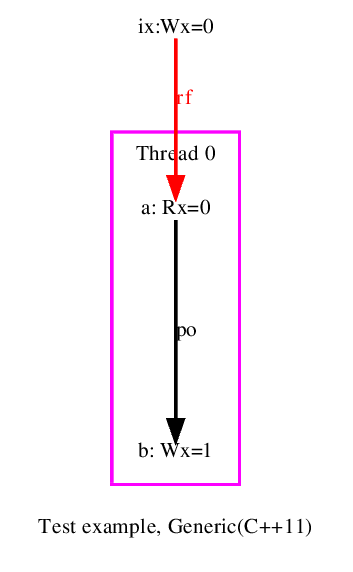
\includegraphics[scale=0.25]{screen}
\caption{A diagram generated from the only possible execution of the previous example}
\end{figure}

%SHOW DIAGRAM

%\section{solution (partielle) proposée, mise en perspective avec l'etat de l'art}

Generating all possible orders is not particularly efficient, on top of this, herd only performs one optimisation : the user can specify a filter on the results which will discard executions before checking them against the .cat model. Because of this .cat is only really useable on fairly small litmus tests and cannot be used to verify real world applications. Traditionally the complexity of model checking for memory models comes from the fact that it is necessary to compute and store a large set of executions which costs a lot of memory or generate them on the fly which incurs the risk of generating the same executions several times. However Michalis Kokologiannakis, Ori Lahav, Konstantinos Sagonas, and Viktor Vafeiadis recently came up with a stateless algorithm for rc11 model checking. This algorithm guarantees that it won't check two equivalent executions up to reordering of independant transitions, as long as the program to check does not feature any RMW operations. Even if the program features RMW operations, the performance of the algorithm is still quite good. I was tasked with implementing this algorithm in herd as a way to expand its possible uses.

\subsection{How the stateless algorithm works}

The stateless algorithm is quite efficient, however this is due in part to its specificity, as it only works for rc11 models. The algorihtm is based on the fact that non sequentially consistent RC11 consistency is monotonous. That is to say, if a given execution is non SC RC11 consistent, then any complete subset of it is as well. This allows us to only build non SC RC11 consistent executions by construction. Sequential consistency is simply checked when a complete execution has been generated. The algorithm also adds events to a given partial execution in a specific order. The algorithm starts with only the initial writes that initialize the variables at 0 and then adds events to this partial execution. The algorithm is always working with a non SC RC11 consistent partial execution : every read reads from a unique write. Thus we need a way to allow reads to read from writes that were added to the execution later. This is achieved by way of a set of revisitable writes.
Roughly speaking the stateless algorithm works recursively by adding the next event to the partial execution at hand, and generating all the possible executions that can include the events and relations from the prior partial execution. To do this it relies on 4 functions :

\begin{itemize}
\item $visit$ takes as arguments a partial execution and a revisit set. It gets the next event to add to the current execution, adds it and then depending on the type of the event calls either itself, $visit\_read$ or $visit\_write$. In the case where there are no more events to add, $visit$ checks that $\psc$ is acyclic and that there are no data races. If psc is acyclic the event is added to the result, otherwise it is discarded. If there is a data race, a flag is set as it would be under normal circumstances in herd.
\item $visit\_read$ takes as arguments a partial execution $e$, a revisit set and the added read $r$. It computes all the possible write events in $e$ that can be read from according to RC11 and for every such write $w$, calls $visit$ on the partial execution modified so that the $r$ reads from $w$.
\item $visit\_write$ takes as arguments a partial execution $e$, a revisit set and the added write $w$. It computes all the positions in the memory order of $e$ that $w$ can be put in then calls $revisit\_reads$ on every partial execution obtained by inserting $w$ in a possible position in $\mo$.
\item $revisit\_reads$ takes as arguments a partial execution $e$, a revisit set $R$ and the write that we were visiting when $revisit\_reads$ was called $w$. It computes every possible subset $s$ of $R$ satisfying certain properties such as that it cannot reach itself within $\po\cup\rf$. It then visits the execution obtained by making all the reads in $s$ read from $w$, removing all the $\po\cup \rf$ successors of $s$ from $e$ and removing all the $\po\cup\rf$ ancestors of $s$ from its revisit set.
\end{itemize}

\section{Translation of rc11 into .cat}

As an introduction to memory models, I implemented rc11 in .cat which had not been done yet, this was quite straightforward as it merely boiled down to translating formulas into .cat and the better part of my time was spent understanding memory models in general as well as the rc11 model in particular.

\section{Implementation of RC11 in herd}

To get familiar with the quite large codebase of herd, I then implemented an rc11 check directly into herd as it would otherwise have been generated from a .cat file. This allowed me to get familiar with how herd was put together and better understand its inner workings, as well as more generally how to work on a large project with many modules spread out over different files.

\section{Implementation of the stateless algorithm in herd}

Once I had become familiar enough with both memory models and herd, I started implementing the stateless algorithm into herd. The stateless algorithm starts with only the initial writes and then adds events in a specific order, I did this by defining a type that stored a set of added events, as well as events to add such that they can be added in a consistent order, relations, the revisit set and some debug information.

The source code of my implementation can be found at :
\begin{lstlisting}
https://github.com/SimonColin/herdtools7
\end{lstlisting}

\subsection{Differences between the stateless algorithm and my implementation}

As stated before, herd makes a choice of branches before calculating executions, since rewriting herd to not do this would have taken quite a bit of time and involved parts of the program that I was not at all familiar with, my current implementation works on each choice of branches, this means that up to any given branching path, it will generate the same set of pre-executions for every choice. This can be quite bad for performance in theory. Another difference is that RMW operations in the current implementation of herd are handled as a single memory event, but the algorithm requires them to be a read and a write, this variant was already implemented for a certain type of RMWs (fetch and increment) but had to be extended to another type (compare and swap) which I did.

%\section{problemes laissés ouverts/points de continuation}

\section{Work still to be done for the stateless algorithm in herd}

I have access to my cat implementation of RC11 and my implementation of the stateless algorithm in herd. This allows me to check my stateless algorithm against the .cat model. For programs without RMWs the stateless algorithm gives the same results as herd using the .cat file, albeit more slowly, but it has yet to be optimised. On a given base of tests, herd using a cat file took a user time of $1m0,805s$ whereas my implementation of the stateless algorithm took $2m43,248s$. As far as programs with RMW operations are concerned, some bugs still persist where the results obtained with the rc11 .cat file and the stateless algorithm differ. I did not have access to the reference implementation by Kokologiannakis, Lahav, Sagonas and Vafeiadis, so I couldn't compare it to herd using a cat model. However they made use of herd to check that their algorithm produced the right results. While doing this they noted that the results produced were the same but that "for the larger [tests] herd was significantly slower.".

\section{SMT solvers for memory model checking}

We recently had a talk with Hernan Ponce de Leon who did some work on using the advances made in the field of smt solvers to perform memory model checking, it would be of interest to enrich herd with this algorithm as well and this would be a possible continuation once the stateless algorithm works and has been optimized.

\end{document}
